\chapter{Enriching the Encoder by Targeting Self-Attention}
\label{enriching}

In this chapter, we present our proposals to enrich the encoder.
In contrast to \citeauthor{sennrich2016linguistic}, we do not simply feed the network with more information, e.g. POS tags or dependency labels, but directly instruct the self-attention mechanism to build upon these types of information.
With this approach, we aim to make the model aware of the source sentence structure and make sure that this happens at the attention layer, the most appropriate layer to deal with relations between tokens.

\cref{enriching-structure} discusses the first approach which introduces dependency-related attentional biases to the \transformer. 
In \cref{enriching-specialized}, we propose a novel specialized attention head guided by syntactic information.

\section{Structured Attentional Bias}
\label{enriching-structure}

With this approach, we make the \transformer model aware of the source sentence structure by introducing bias terms which are similar to the relative position, but based on the dependency tree.

% \subsection{Relative Position}
% \label{enriching-structure-relative}

Let us recall the formula to compute the attention energy $e_{ij}$ (before the softmax layer to get attention weight $a_{ij}$):

\begin{equation}
    e_{ij}=\frac{1}{\sqrt{d_k}} x_i W^Q (x_j W^K)^\top
\end{equation}

The energy $e_{ij}$ is simply a dot product of the query $q_i=x_i W^Q$ (input $x_i$ projected through $W^Q$) and the key $k_j=x_j W^K$ (input $x_j$ projected through $W^K$) and divided by the square root of the attention hidden size $d_k$.
The formula above assumes that the positional encoding has been included in the input.
However, this positional encoding is generated from the absolute position of a token within the sentence. \cite{DBLP:conf/naacl/ShawUV18} proposed to impose the encoding of \textit{relative position} in the attention layer instead by adding a bias term:

\begin{equation}
    e_{ij}=\frac{1}{\sqrt{d_k}} x_i W^Q (x_j W^K + b^K_{ij})^\top
\end{equation}

The bias term $b^K_{ij}$ is the embedding vector of the relative position label between token $i$ and $j$. \cref{fig:relative-position-label} illustrates this type of labels between token ``is" and its neighbors in a sample sentence.
These relative position labels are considered as discrete symbols, whose embeddings can be learned the same way as word embeddings.

\begin{figure}[t]
    \centering
    \begin{dependency}
        \begin{deptext}
        I \& think \& this \& is \& a \& good \& idea \& . \\
        \end{deptext}
        \depedge{4}{1}{-3}
        \depedge{4}{2}{-2}
        \depedge{4}{3}{-1}
        \depedge{4}{5}{1}
        \depedge{4}{6}{2}
        \depedge{4}{7}{3}
        \depedge{4}{8}{4}
    \end{dependency}
    \caption{Relative position labels of the token \textit{is} and its neighbors.}
    \label{fig:relative-position-label}
\end{figure}

Following \citeauthor{DBLP:conf/naacl/ShawUV18}, we also enrich the encoder's attention function by introducing structural biases.
Instead of the relative position, we would like to use the information from the source-side dependency tree.
We experiment with two forms of these labels: tree distance and tree traversal encoding.

\subsection{Tree Distance}
\label{enriching-structure-treedist}

Our first proposal is the distance between two nodes in a dependency tree, i.e. the number of edges connecting the two nodes. Our model \TreeDistance utilizes this distance embedding as the bias term $t_{ij}^K$ instead of the relative position bias $b^K_{ij}$, or in a combination of both:

\begin{equation}
 e_{ij}=\frac{1}{\sqrt{d_k}} x_i W^Q (x_j W^K + b^K_{ij} + t_{ij}^K)^\top
\end{equation}

\cref{fig:tree-relative-distance} shows how we obtain the tree distance labels from a dependency tree.
In this example, the distance between \textit{is} and \textit{think} is $1$, because there is one edge connecting them.
On the other hand, \textit{is} and \textit{a} is two edges apart, so the tree distance label is $2$.
It is obvious that this tree distance label is symmetrical, i.e. the tree distance between $i$ and $j$ is identical to the tree distance between $j$ and $i$.

To be able to learn the embeddings, the model has to limit the maximum distance to maintain a fixed-size set of these labels. All token pairs that exceed this maximum distance are assigned a special label, which is similar to the out-of-vocabulary token (\texttt{<OOV>}).

\begin{figure}[t]
    \centering
    \begin{forest}
    dg edges
    [ROOT
        [think, edge={<-}, edge label={node[midway,fill=white] {2}}
          [I, edge={->}, edge label={node[midway,fill=white] {2}} [I]] 
          [think]
          [\textbf{is}, red, edge={<-}, edge label={node[midway,fill=white] {1}}
          	[this, edge={->}, edge label={node[midway,fill=white] {1}} [this]]
            [is]
            [idea, edge={->}, edge label={node[midway,fill=white] {1}}
            	[a, edge={->}, edge label={node[midway,fill=white] {2}} [a]]
                [good, edge={->}, edge label={node[midway,fill=white] {2}} [good]]
                [idea]
            ]
          ]
        ]
        [., edge={->}, edge label={node[midway,fill=white] {3}} [.]]
    ]
    \end{forest}
    \caption{Example of tree distance labels of token \textit{is} and the other tokens in a dependency tree. The arc label expresses the tree distance from \textit{is} to the node at the tail of the arc.}
    \label{fig:tree-relative-distance}
\end{figure}

\subsection{Tree Traversal Encoding}
\label{enriching-structure-treetraversal}

We also expand the simple numerical tree distance above into the tree traversal encoding.
This encoding does not only describe the distance but also the path from one node to another.
Our model \TreeTraversal makes use of this encoding the same way the \TreeDistance model utilizes the tree distance label.

\cref{fig:tree-traversal-encoding} elaborates our idea in a more intuitive way.
Let us get back to the token \textit{is}, to traverse from \textit{is} to \textit{ROOT}, we need to go up (\textit{U}) twice. 
Hence, the traversal encoding from \textit{is} to \textit{ROOT} is ``\textit{UU}".
It is important to note that while the tree distance is symmetrical, tree traversal encoding is not.
This is because the direction of the path from \textit{is} to \textit{ROOT} is different from the path from \textit{ROOT} to \textit{is}.

\begin{figure}[t]
    \centering
    \begin{forest}
    dg edges
    [ROOT
        [think, edge={<-}, edge label={node[midway,fill=white] {UU}}
          [I, edge={->}, edge label={node[midway,fill=white] {L}} [I]] 
          [think]
          [\textbf{is}, red, edge={<-}, edge label={node[midway,fill=white] {U}}
          	[this, edge={->}, edge label={node[midway,fill=white] {D}} [this]]
            [is]
            [idea, edge={->}, edge label={node[midway,fill=white] {D}}
            	[a, edge={->}, edge label={node[midway,fill=white] {DD}} [a]]
                [good, edge={->} [good]]
                [idea]
            ]
          ]
        ]
        [., edge={->}, edge label={node[midway,fill=white] {UUD}} [.]]
    ]
    \end{forest}
    \caption{Example of tree traversal encodings of token \textit{is} and the other tokens in a dependency tree. The arc label expresses the tree traversal encoding from \textit{is} to the node at the tail of the arc.}
    \label{fig:tree-traversal-encoding}
\end{figure}

In addition to the two characters `\textit{U}' (up) and `\textit{D}' (down), we also add two special characters to denote the path from the current node to its siblings: `\textit{L}' for its left siblings and `\textit{R}' for its right siblings.
In \cref{fig:tree-traversal-encoding}, the traversal encoding from \textit{is} to \textit{I} is ``\textit{L}" instead of ``\textit{UD}", because \textit{I} is the left sibling of \textit{is}.
Sibling notation takes precedence over `U' and `D' but it is limited to siblings of the current node.

The maximum length of this traversal encoding ($max\_traversal$) is also restricted in order to have a fixed-size vocabulary of the traversal encodings.
% This restriction allows the model learn the embeddings better.
Moreover, the size of the vocabulary generated from our tree traversal does not grow exponentially to $max\_traversal$ because the encoding should be of the shortest path between two nodes in the tree. Hence, all possible encodings can be matched with the following regular expressions:
\begin{itemize}
    \item \textbf{U*D*} : go all the way up (or not) and then down (or not).
    \item \textbf{LD*}      : to the left sibling then down.
    \item \textbf{RD*}      : to the right sibling then down.
\end{itemize}

There is no reason to go down then up (e.g. ``DDDDUU") because a shorter encoding with only `D' characters can encode this path (``DD").

\section{Specialized Attention Heads}
\label{enriching-specialized}

In a normal self-attention layer (\cref{lit-trans-att}), the input $x_i$ is projected through three matrices $W^Q, W^K, W^V$ to obtain the corresponding key, query and value vectors.
The reason for these projections, as discussed in the previous section, is to allow the key, query and value to come from various representation subspaces.

We hypothesize that it may be beneficial for the model that one of these vectors truly come from a known representation space even before the projection.
To be specific, at the shallowest layer (layer 0) of the encoder, we propose the value to be projected from the token embedding (as in the standard \transformer), but the key and query should be projected from some linguistic label embeddings, e.g. POS tags or dependency labels.

As illustrated in \cref{fig:specialized-heads}, the input $x_i$ (token embedding on layer 0) is solely projected to the value vector $v_i$, while the query $q_i$ and key $k_i$ are obtained by projecting an additional input sequence $l_i$ (POS embedding).
Because the attention is guided by this supplementary information $l_i$, we would like to call it a ``specialized attention head".

\begin{figure}[t]
    \centering
    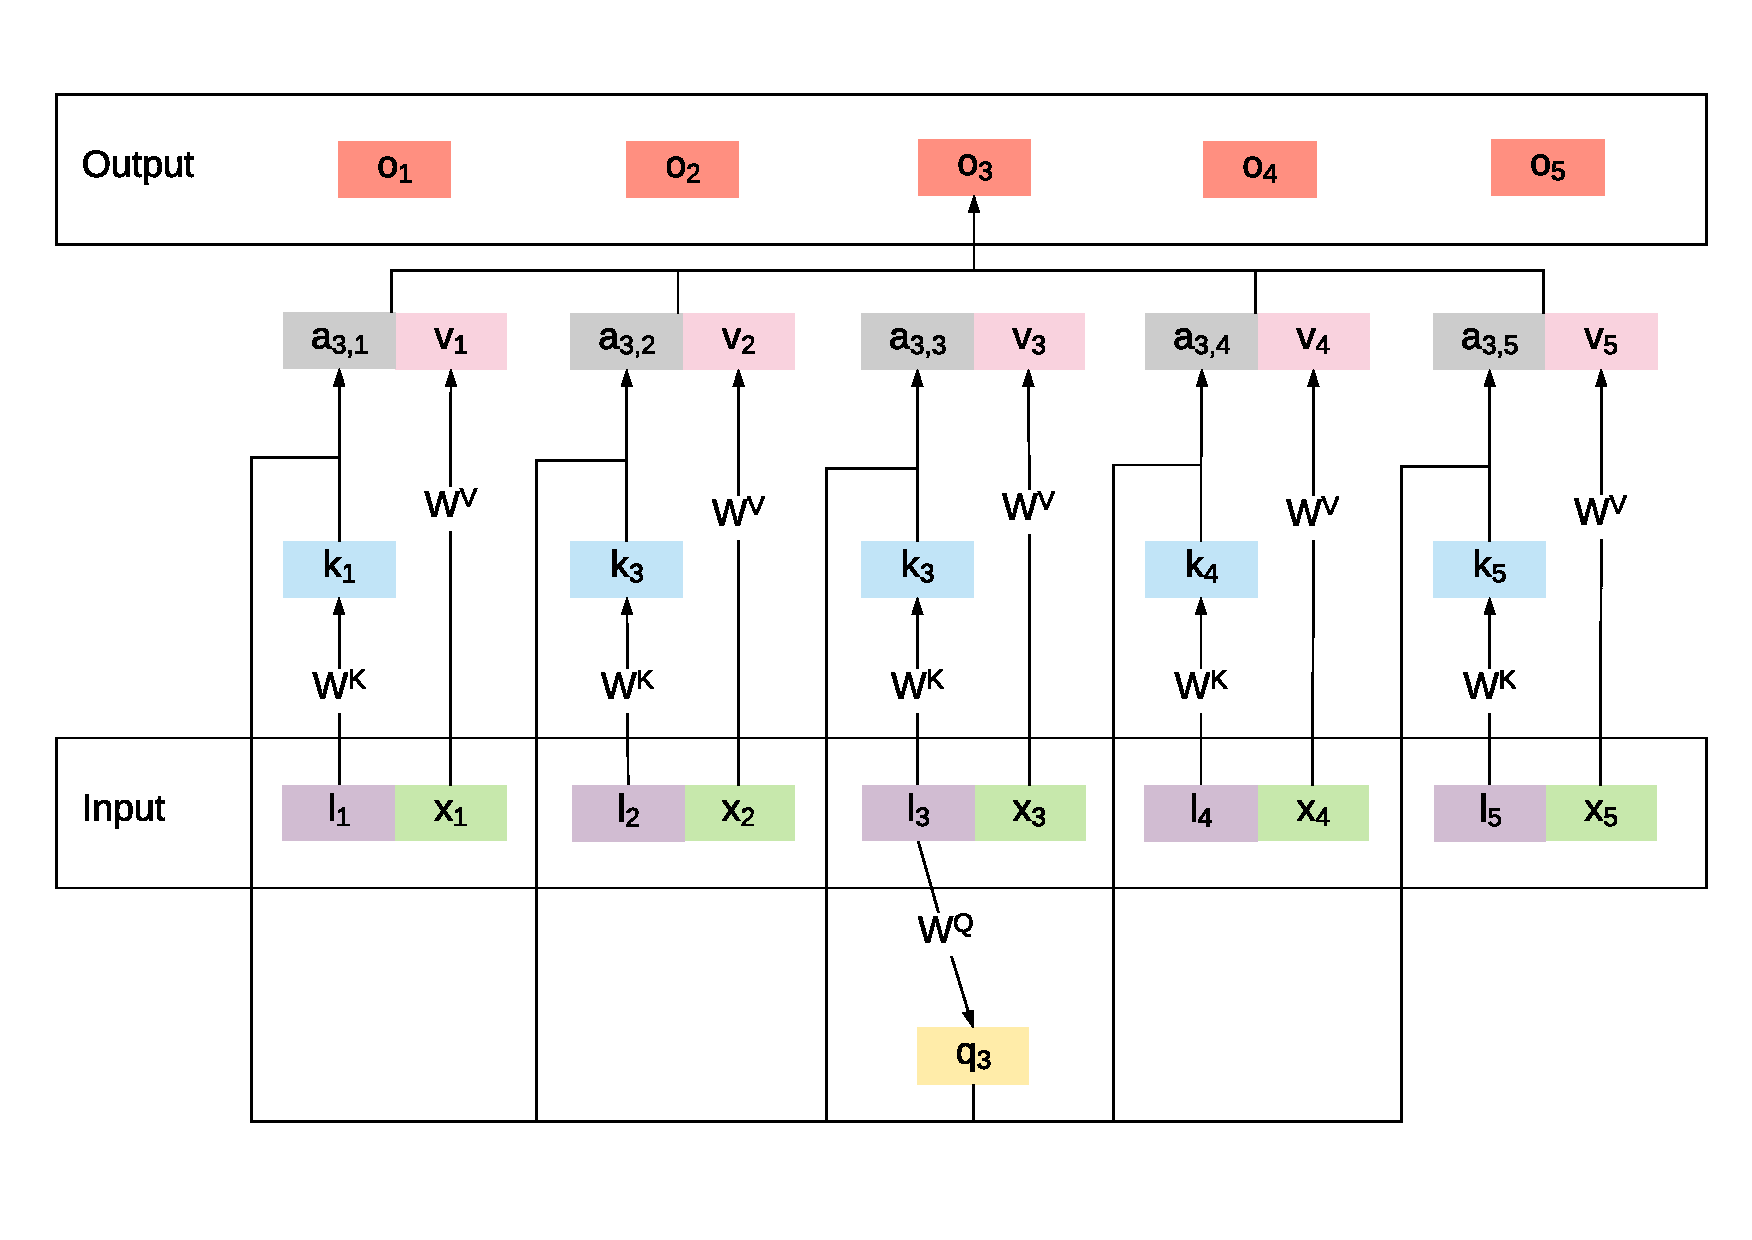
\includegraphics[width=\linewidth]{img/specialized-head.pdf}
    \caption{Specialized attention head with POS tag embeddings as keys and queries, computing the output $o_3$.}
    \label{fig:specialized-heads}
\end{figure}

In our experiment, we only apply this specialized attention in one head of the shallowest layer in the encoder.
In this chosen head, the model will calculate the self-attention weights with keys $k_i$ and queries $q_i$ from one of the following linguistic labels:

\begin{itemize}
	\item POS embeddings (\SpecPOS, \cref{fig:specialized-heads}).
    \item Dependency label embeddings (\SpecDep, $l_i$ is dependency label embedding instead).
\end{itemize}

% instead of token embeddings. Hence, the $l_i$ in \cref{fig:specialized-heads} is either POS tag embeddings or dependency label embeddings.
